\documentclass{article}
\usepackage{setspace}
\usepackage{geometry}
\usepackage[utf8]{inputenc}
\usepackage{amsmath,amsthm,amssymb,bm}
\usepackage{mathtools}

\geometry{letterpaper, portrait, margin=1in}
\setstretch{1.5}
\title{Homework 6}
%\date{1-18-2020}
\author{Runmin Lu}

\begin{document}
	\maketitle
	%\newpage
	
	\section*{Exercise 3.4}
	\subsection*{(a)}
		\begin{align*}
			\hat{\mathbf y} &= \mathbf X \mathbf w_{\text{lin}}\\
			&= \mathbf X(\mathbf X^T\mathbf X)^{-1}\mathbf X^T\mathbf y\\
			&= \mathbf X(\mathbf X^T\mathbf X)^{-1}\mathbf X^T(\mathbf X\mathbf w^* + \bm\epsilon)\\
			&= \mathbf X(\mathbf X^T\mathbf X)^{-1}\mathbf X^T\mathbf X\mathbf w^* + \mathbf X(\mathbf X^T\mathbf X)^{-1}\mathbf X^T \bm\epsilon\\
			&= \mathbf{Xw}^* + \mathbf H\bm\epsilon
		\end{align*}
	\subsection*{(b)}
		\begin{align*}
			\hat{\mathbf y} - \mathbf y &= \mathbf{Xw}^* + \mathbf H\bm\epsilon - (\mathbf{Xw}^* + \bm\epsilon)\\
			 &= \mathbf H\bm\epsilon - \bm\epsilon\\
			 &= (\mathbf H - \mathbf I)\bm\epsilon
		\end{align*}
	\subsection*{(c)}
		\begin{align*}
			E_\text{in}(\mathbf w_{\text{lin}}) &= \frac1N\sum\limits_{i=1}^N(\hat y_i - y_i)^2\\
			&= \frac1N||\hat{\mathbf y} - \mathbf y||^2\\
			&= \frac1N||(\mathbf H - \mathbf I)\bm\epsilon||^2\\
			&= \frac1N||(\mathbf I - \mathbf H)\bm\epsilon||^2\\
			&= \frac1N\bm\epsilon^T(\mathbf I - \mathbf H)^T(\mathbf I - \mathbf H)\bm\epsilon\\
			&= \frac1N\bm\epsilon^T(\mathbf I - \mathbf H)^2\bm\epsilon\\
			&= \frac1N\bm\epsilon^T(\mathbf I - \mathbf H)\bm\epsilon\\
		\end{align*}
		
	\subsection*{(d)}
		\begin{align*}
			\mathbb E_{\mathcal D}[E_\text{in}(\mathbf w_{\text{lin}})] &= \mathbb E_{\mathcal D}[ \frac1N\bm\epsilon^T(\mathbf I - \mathbf H)\bm\epsilon ]\\
			&= \frac1N\mathbb E_{\mathcal D}[ \bm\epsilon^T(\mathbf I - \mathbf H)\bm\epsilon ]\\
			&= \frac1N\mathbb E_{\mathcal D}[ \bm\epsilon^T\bm\epsilon - \bm\epsilon^T\mathbf H\bm\epsilon ]\\
			&= \frac1N(\mathbb E_{\mathcal D}[||\bm\epsilon||^2] - \mathbb E_{\mathcal D}[\bm\epsilon^T\mathbf H\bm\epsilon])\\
			\mathbb E_{\mathcal D}[||\bm\epsilon||^2] &= \sum\limits_{i=1}^N\mathbb E_{\mathcal D}[\epsilon_i^2]\\
			&=N\sigma^2\\
			\bm\epsilon^T\mathbf H\bm\epsilon &= \sum\limits_{i=1}^N\sum\limits_{j=1}^NH_{ij}\epsilon_i\epsilon_j\\
			\mathbb E_{\mathcal D}[\epsilon_i\epsilon_j] &=
			\begin{cases}
				\sigma^2 &i = j\\
				0 &i \neq j \ \ \ \ \ (\epsilon_i, \epsilon_j \text{ are independent})
			\end{cases}\\
			\mathbb E_{\mathcal D}[\bm\epsilon^T\mathbf H\bm\epsilon] &= \sum\limits_{i = 1}^NH_{ii}\sigma^2\\
			&= \sigma^2\text{trace}(\mathbf H)\\
			&= \sigma^2(d+1)\\
			\mathbb E_{\mathcal D}[E_\text{in}(\mathbf w_{\text{lin}})] &= \frac1N(N\sigma^2 - \sigma^2(d+1))\\
			&= \sigma^2(1 - \frac{d+1}N)
		\end{align*}
		
	\subsection*{(e)}
		\begin{align*}
			\mathbf y' &= \mathbf X\mathbf w^* + \bm\epsilon'\\
			\hat{\mathbf y} - \mathbf y' &= \mathbf{Xw}^* + \mathbf H\bm\epsilon - (\mathbf{Xw}^* + \bm\epsilon')\\
			&= \mathbf H\bm\epsilon - \bm\epsilon'\\
			E_\text{test}(\mathbf w_{\text{lin}}) &=\frac1N||\hat{\mathbf y} - \mathbf y'||^2\\
			&= \frac1N||\mathbf H\bm\epsilon - \bm\epsilon'||^2\\
			&= \frac1N(\bm\epsilon^T\mathbf H^T\mathbf H\bm\epsilon - 2\bm\epsilon'^T\mathbf H\bm\epsilon + ||\bm\epsilon'||^2)\\
			&= \frac1N(\bm\epsilon^T\mathbf H\bm\epsilon - 2\bm\epsilon'^T\mathbf H\bm\epsilon + ||\bm\epsilon'||^2)\ \ \ \ \ (\text{from Exercise 3.3 (b)})\\
			\mathbb E_{\mathcal D, \bm\epsilon'}[E_\text{test}(\mathbf w_{\text{lin}})] &= \frac1N(\mathbb E_{\mathcal D, \bm\epsilon'}[\bm\epsilon^T\mathbf H\bm\epsilon] - \mathbb E_{\mathcal D, \bm\epsilon'}[2\bm\epsilon'^T\mathbf H\bm\epsilon] + \mathbb E_{\mathcal D, \bm\epsilon'}[||\bm\epsilon'||^2])\\
			\bm\epsilon'^T\mathbf H\bm\epsilon &= \sum\limits_{i=1}^N\sum\limits_{j=1}^NH_{ij}\epsilon_i'\epsilon_j\\
			\mathbb E_{\mathcal D, \bm\epsilon'}[\epsilon_i'\epsilon_j] &= 0\ \ \ \ \ (\epsilon_i', \epsilon_j \text{ are independent})\\
			\mathbb E_{\mathcal D, \bm\epsilon'}[\bm\epsilon'^T\mathbf H\bm\epsilon] &= 0\\
			\mathbb E_{\mathcal D, \bm\epsilon'}[E_\text{test}(\mathbf w_{\text{lin}})] &= \frac1N(\mathbb E_{\mathcal D, \bm\epsilon'}[\bm\epsilon^T\mathbf H\bm\epsilon] + \mathbb E_{\mathcal D, \bm\epsilon'}[||\bm\epsilon'||^2]\\
			&=\frac1N(\sigma^2(d+1) + N\sigma^2)\\
			&= \sigma^2(1 + \frac{d+1}N)
		\end{align*}
		
	\section*{Problem 3.1}
	\subsection*{(a)}
		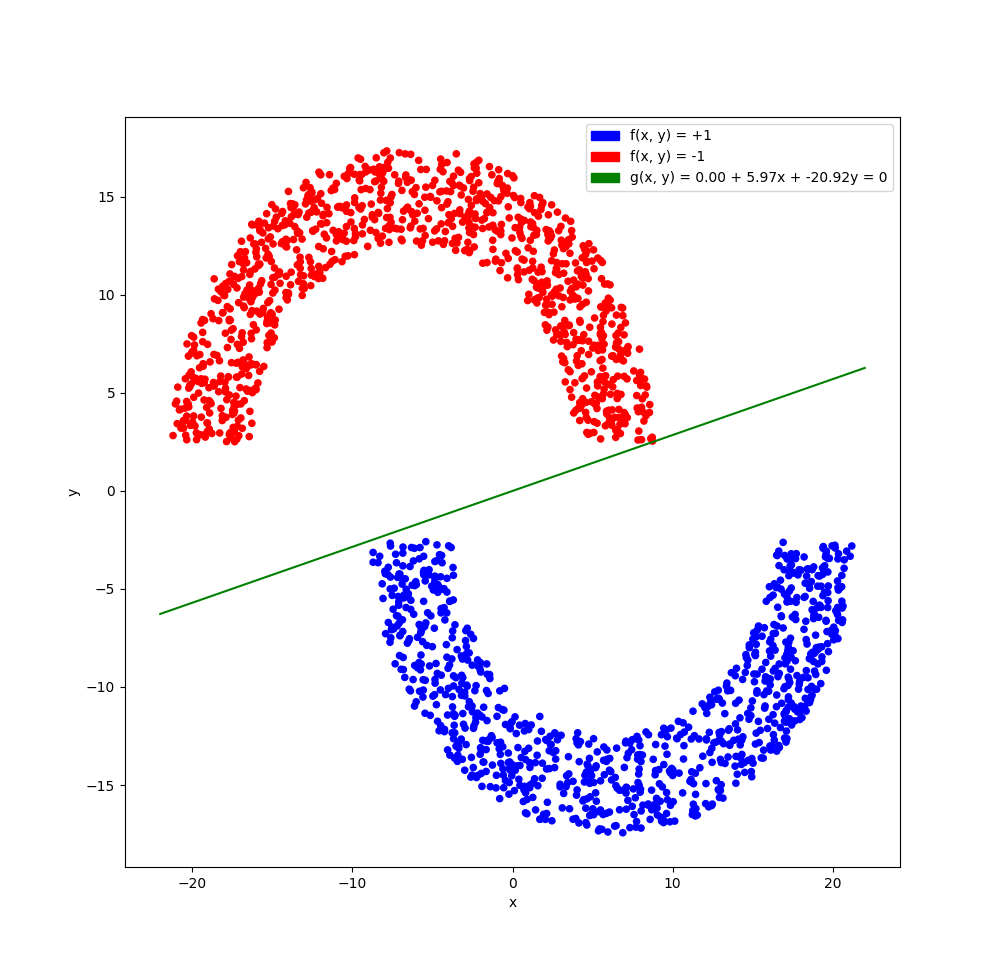
\includegraphics[scale=0.38]{p3.1a.png}
	\subsection*{(b)}
		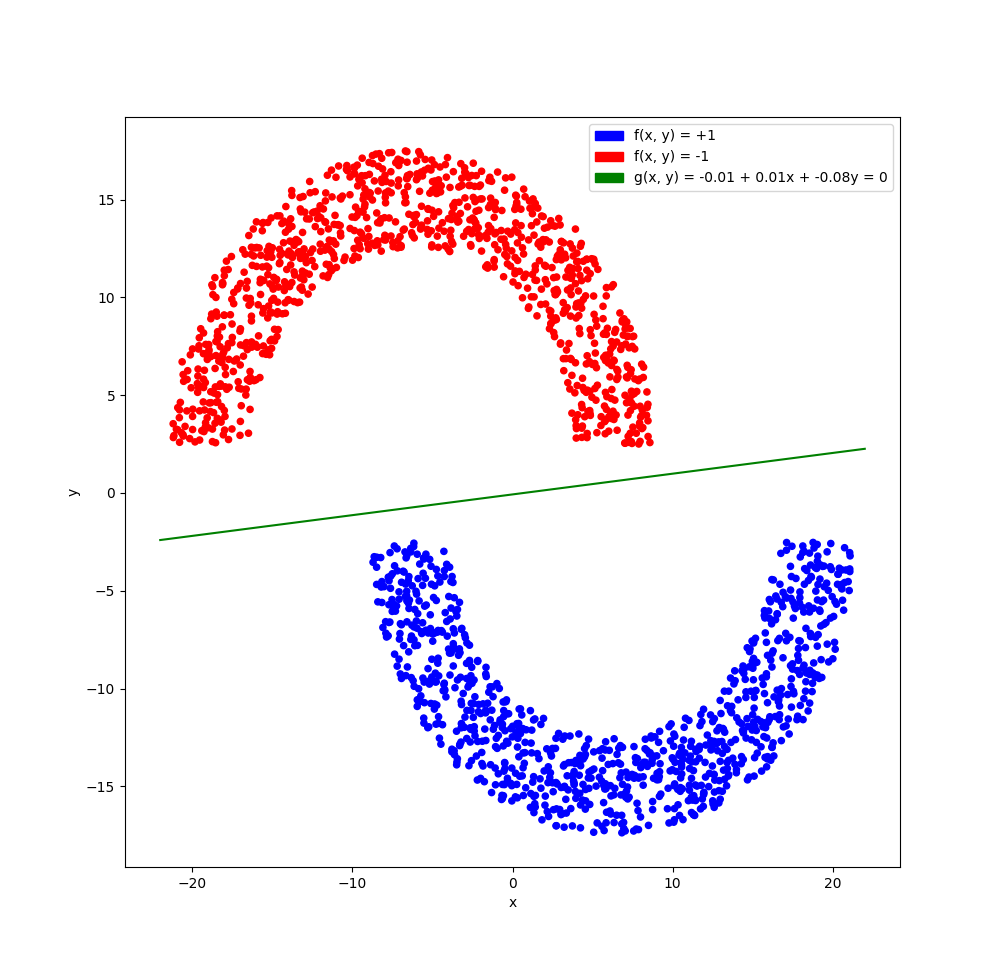
\includegraphics[scale=0.38]{p3.1b.png}\\
		If you run this perceptron and regression multiple times, the weight vector generated by regression is a lot more consistent than the one for perceptron. The reason behind this is that regression is deterministic: $\mathbf w_\text{lin}$ only depends on the data points. On the other hand, $\mathbf w$ generated by preceptron also depends on the order we update it. In each iteration, we can have multiple options of misclassified points to update the weight with, which can result in many possible subsequent weight.
		
	\section*{Problem 3.2}
		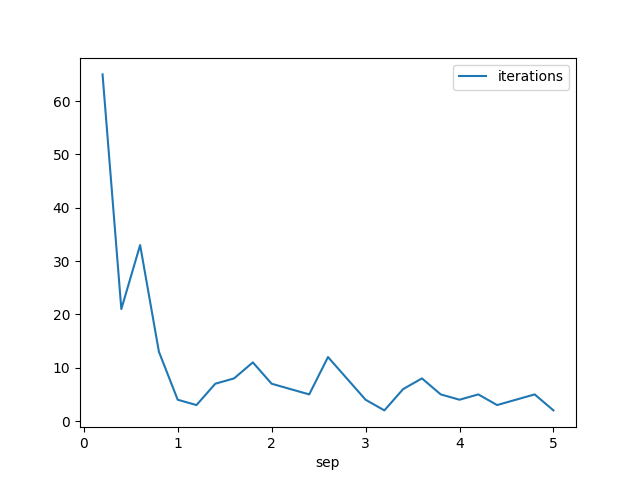
\includegraphics[scale=0.7]{p3.2.png}\\
		As $sep$ increases, the number of iterations it takes to converge generally decreases. From Problem 1.3, we know that $t \leq \frac{R^2||\mathbf w^*||^2}{\rho^2}$ where $\rho = \min\limits_{1 \leq n \leq N}y_n(\mathbf w^{*T} \mathbf x_n)$. As $sep$ increases, all the $\mathbf x_n$'s are farther from the origin, which means that their norms increase, $\mathbf w^{*T} \mathbf x_n$ also increases in absolute value, $rho$ increases, and the upper bound for $t$ decreases since $\rho^2$ is in the denominator.
		
	\section*{Problem 3.8}
		Suppose for contradiction that there's some $h'(\mathbf x) = \mathbb E[y | \mathbf x] + \epsilon(\mathbf x)$ that gives an even smaller $E_\text{out}$, where $\epsilon(\mathbf x)$ is some aribtrary deterministic function of $\mathbf x$.\\
		Then
		\begin{align*}
			E_\text{out}(h') - E_\text{out}(h^*) &= \mathbb E[ (\mathbb E[y | \mathbf x] + \epsilon(\mathbf x) - y)^2] - \mathbb E[ (\mathbb E[y | \mathbf x] - y)^2]\\
			&= \mathbb E[(\mathbb E[y|\mathbf x] - y)^2 + 2\epsilon(\mathbf x)(\mathbb E[y|\mathbf x] - y) + \epsilon(\mathbf x)^2]  \mathbb E[ (\mathbb E[y | \mathbf x] - y)^2]\\
			&= \mathbb E[(\mathbb E[y|\mathbf x] - y)^2] + \mathbb E[2\epsilon(\mathbf x)(\mathbb E[y|\mathbf x] - y)] + \mathbb E[\epsilon(\mathbf x)^2] - \mathbb E[ (\mathbb E[y | \mathbf x] - y)^2]\\
			&= \mathbb E[2\epsilon(\mathbf x)(\mathbb E[y|\mathbf x] - y)] + \mathbb E[\epsilon(\mathbf x)^2]\\
			&= 2\epsilon(\mathbf x)\mathbb E[\mathbb E[y|\mathbf x] - y] + \mathbb E[\epsilon(\mathbf x)^2]\ \ \ \ \ \text{because }\epsilon(\mathbf x)\text{ is deterministic}\\
			&= \mathbb E[\epsilon(\mathbf x)^2]\ \ \ \ \ \text{because } y \text{ is expected to equal }E[y | \mathbf x] \text{ so } \mathbb E[\mathbb E[y|\mathbf x] - y] = 0\\
			&\geq 0
		\end{align*}
		$E_\text{out}(h')$ is always at least $E_\text{out}(h^*)$ so $h^*$ gives the minimum $E_\text{out}$.
		\begin{align*}
			E_\text{out}(h^*) &= \mathbb E[(h^*(\mathbf x) - y)^2]\\
			&= \mathbb E[(h^*(\mathbf x) - (h^*(\mathbf x) + \epsilon(\mathbf x)))^2]\\
			&= \mathbb E[\epsilon(\mathbf x)^2]
		\end{align*}
		To minimize $E_\text{out}$, we need
		\begin{align*}
			\frac{dE_\text{out}}{d\epsilon} &= 0\\
			\mathbb E[2\epsilon(\mathbf x)] &= 0\\
			E[\epsilon(\mathbf x)] &= 0
		\end{align*}
	\section*{6}
	\subsection*{(a)}
		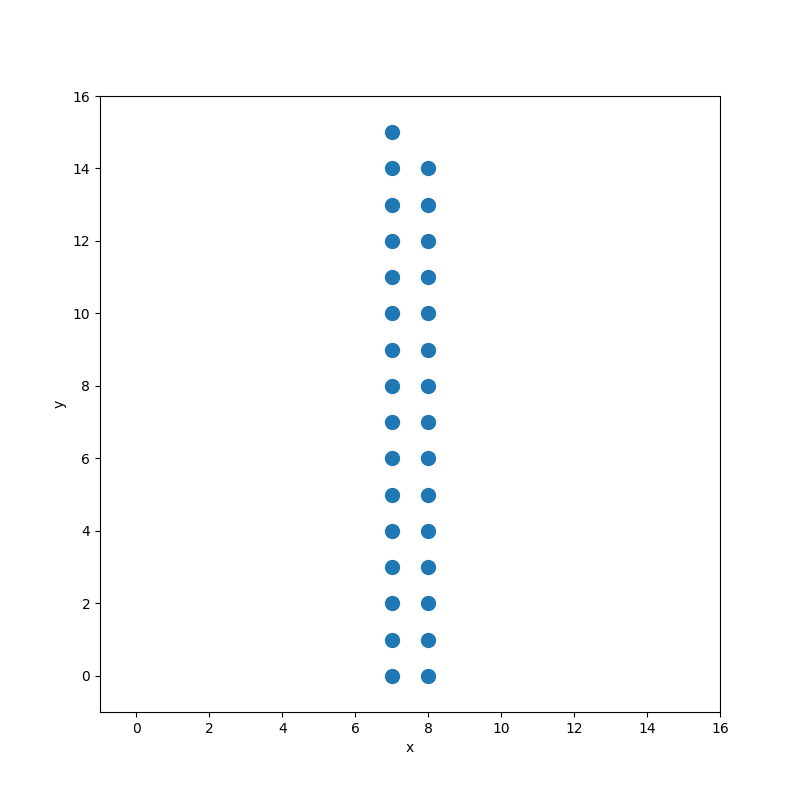
\includegraphics[scale=0.4]{1.png}
		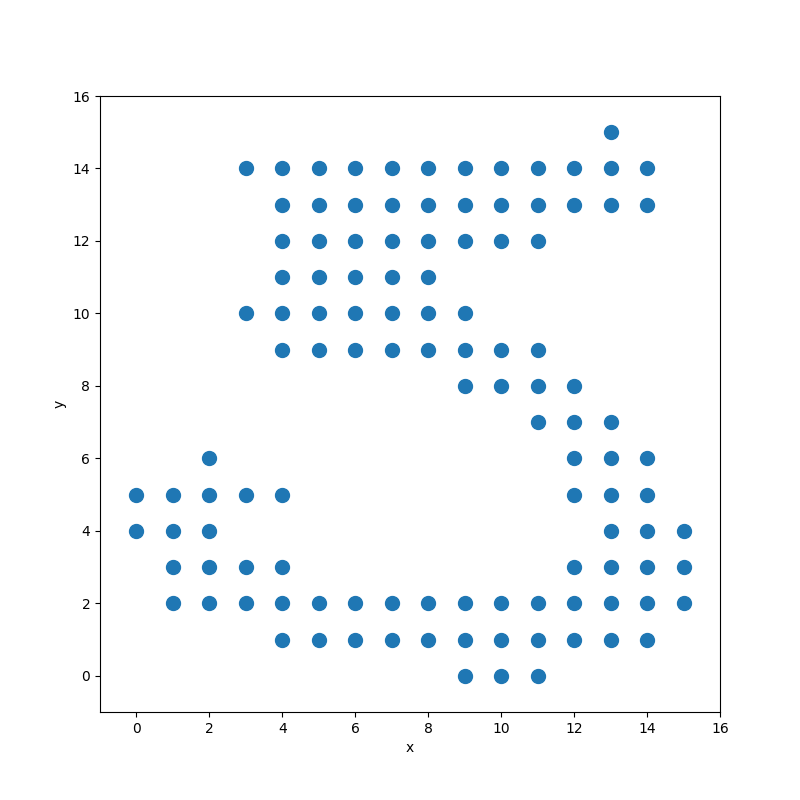
\includegraphics[scale=0.4]{5.png}
	
	\subsection*{(b)}
		The first feature is bounding box area $A$: the area of the smallest axis rectangle that contains all the non-white pixels.\\
		Suppose the set of non-white pixels is $\{(x_1, y_1), ..., (x_n, y_n)\}$.\\
		Then $A = (\max\limits_ix_i - \min\limits_ix_i)(\max\limits_iy_i - \min\limits_iy_i)$\\\\
		The second feature is curviness, which is measured by the following algorithm.\\
		Loop over all the boundary non-white pixels and compute the angle formed by each triple (prev, curr, next) and take the absolute value of  difference of that and $\pi$ (straight means no curve). In practice, we take $\frac \pi 4$ as 1 unit of angle and it doesn't affect the result of learning because scaling is linear.\\
		Sum up all of them to generate the curviness.
	\subsection*{(c)}
		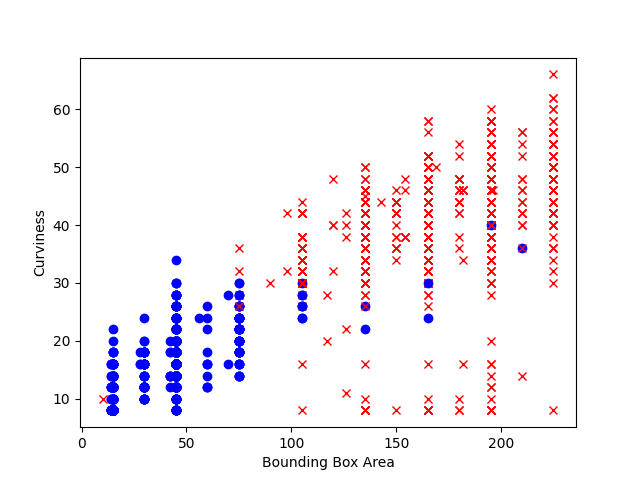
\includegraphics[scale=0.9]{6c.png}\\
		Note: I don't know why but when I give a marker of 'o' it gets filled.
\end{document}